\chapter{Modelo de domínio e dicionário dos dados}

\hspace{5mm} Neste capítulo apresenta-se o modelo de dóminio do sistema bem como é detalhado cada entidade do modelo de dóminio através de um dicionário. Através destes dois modelos é feito um estudo ainda mais profundo e preciso sobre o domínio do sistema, tornando facilitado o processo de deteção de contradições ou ambiguidades e consequentemente é facilitado também o futuro processo de implementação.

\newpage
\section{Modelo de domínio}

\hspace{5mm} Na seguinte figura encontra-se o modelo de domínio criado pelo grupo.

\begin{figure}[H]
    \centering
	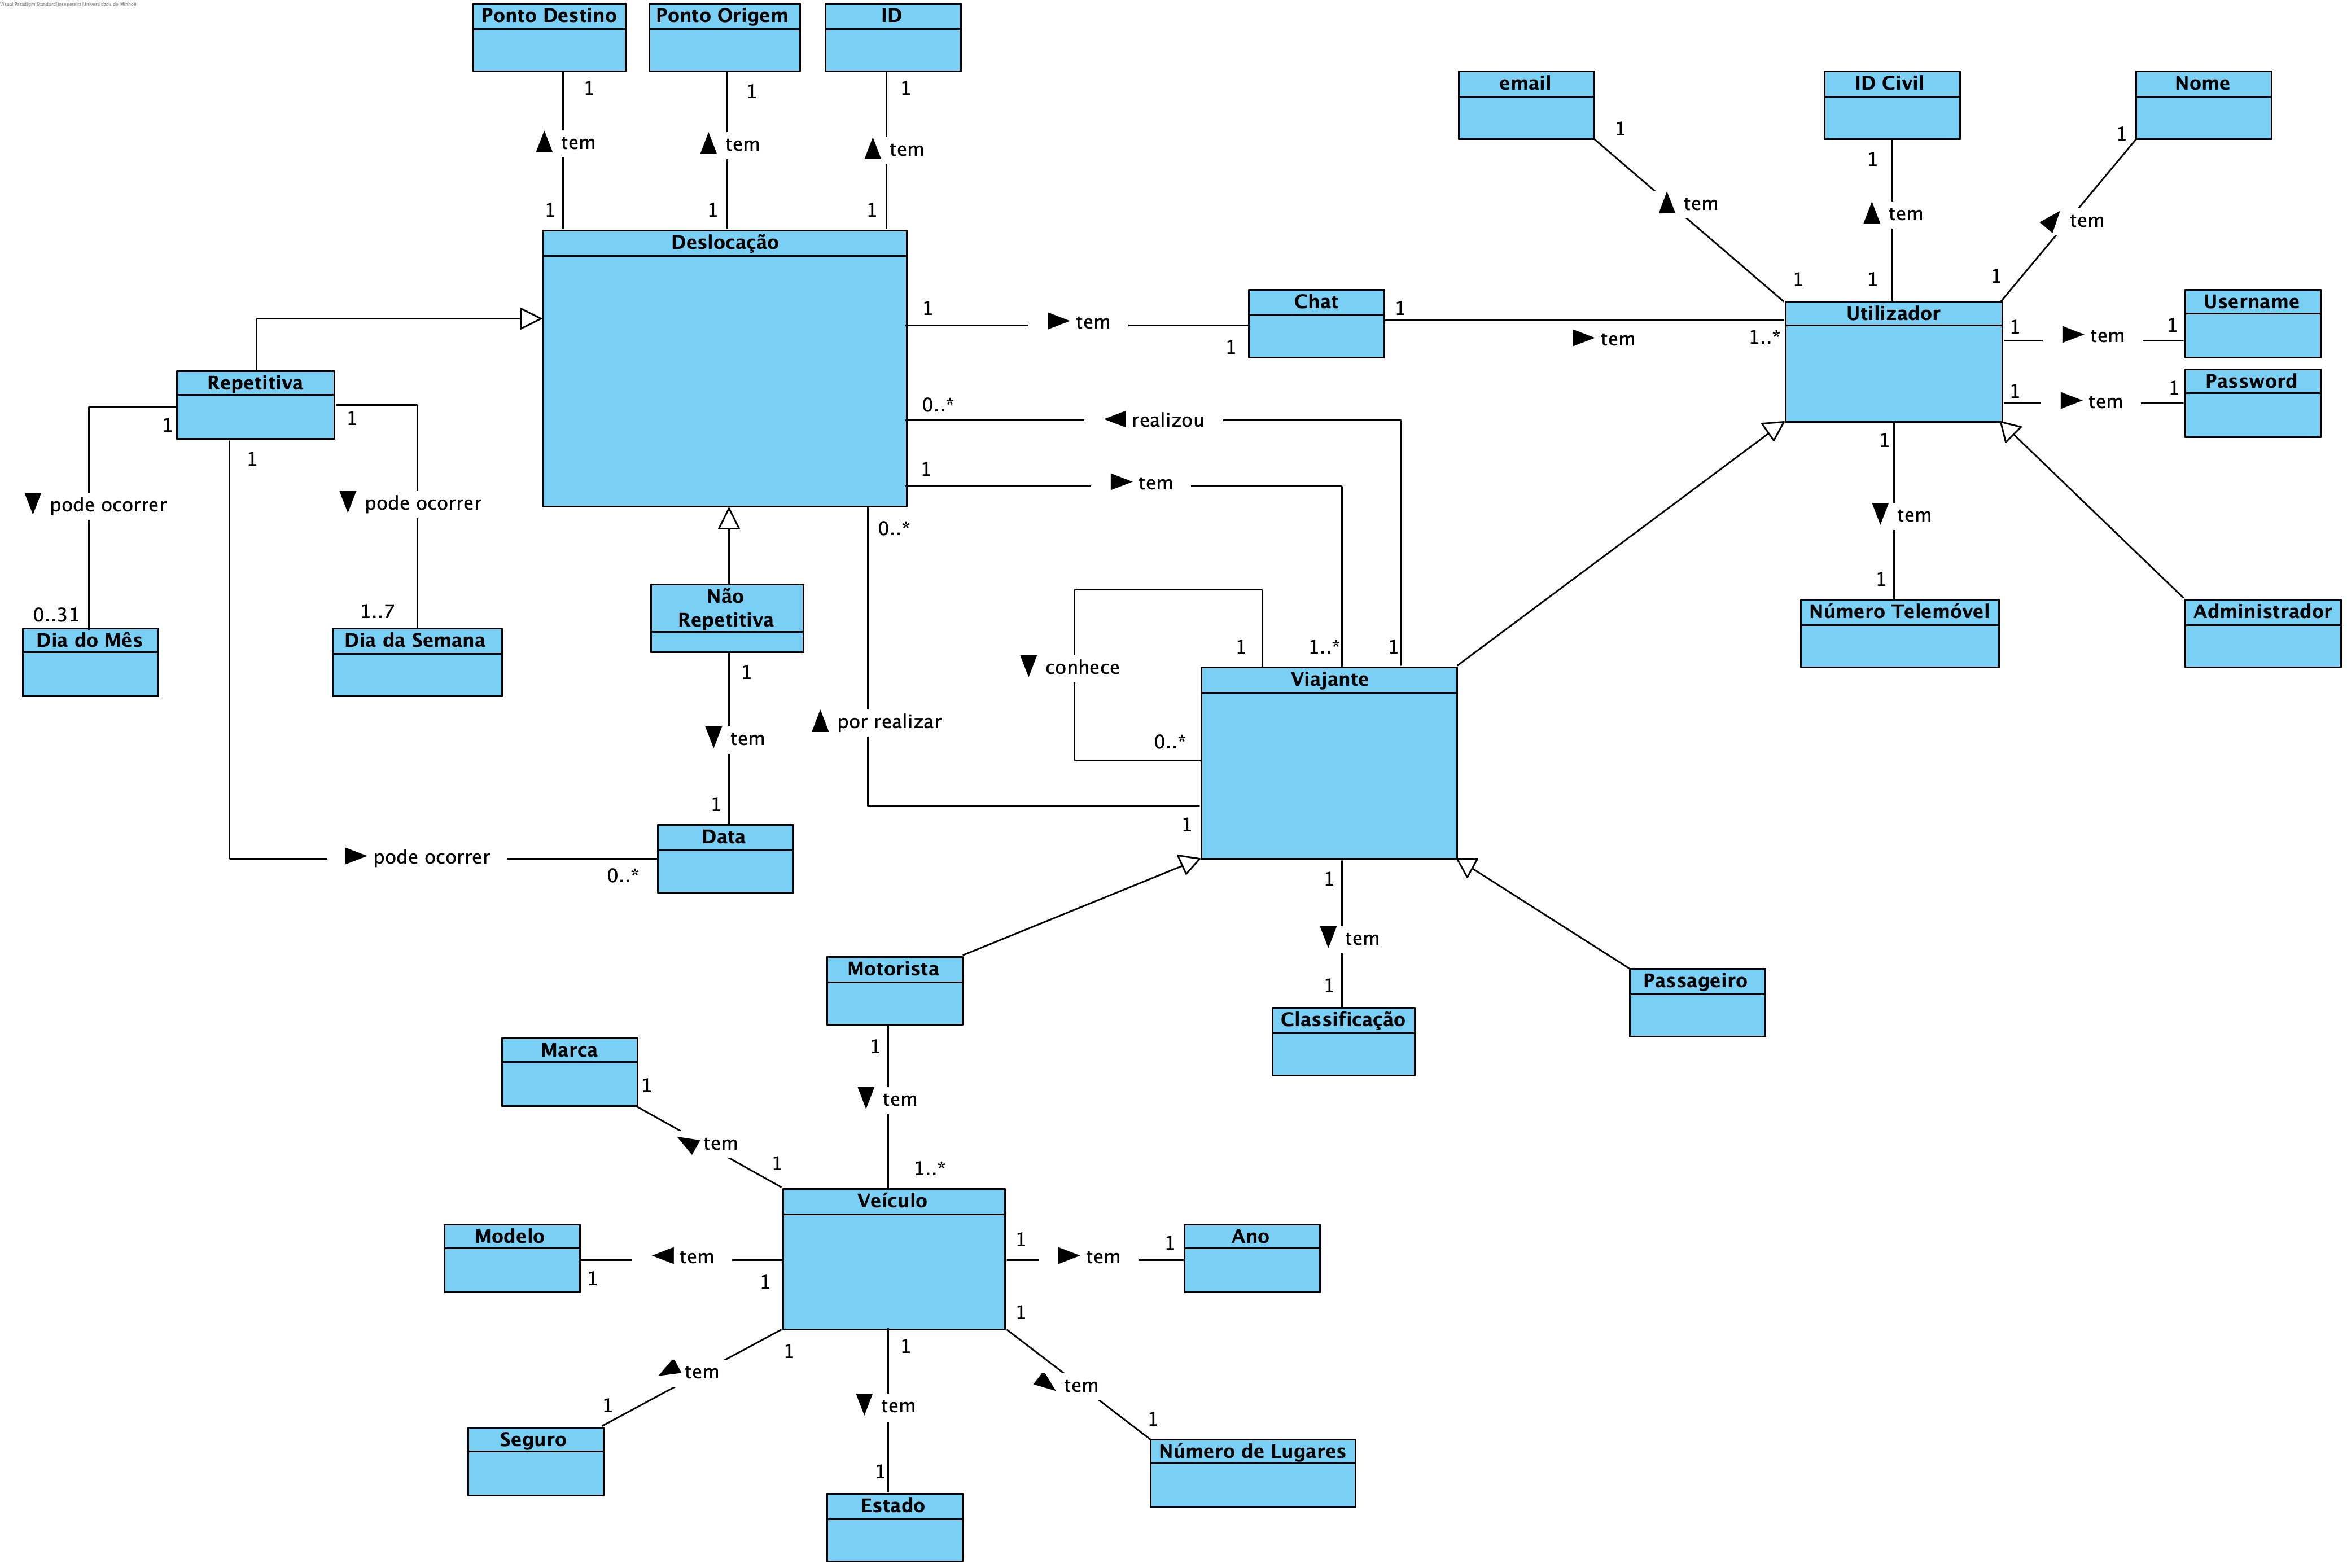
\includegraphics[scale=0.5]{imagens/modelo-dominio.png}
	\label{img:duc1}
	\caption{Modelo de dóminio do sistema.}
\end{figure}

\hspace{5mm} Inicialmente foi introduzida a noção de \textbf{utilizador} que necessita de um \textbf{username} e \textbf{password} para se autenticar no sistema, este é tratado pelo seu \textbf{nome}, pode ser contactado pelo \textbf{email} ou \textbf{número de telemóvel}, por questões de segurança também é identificado pelo seu \textbf{id civil}. 

\hspace{5mm} Desta forma existem dois tipos de utilizador: \textbf{adiministrador} ou \textbf{viajante}. Note-se que a realação entre estes dois últimos e o utilizador é de \textbf{hierarquia}, logo toda a constituição do utilizador encontra-se também no adiministrador e viajante.

\hspace{5mm} O administrador tem o papel de controlar o sistema por isso a sua \textbf{constituição não é maior} que a do utilizador, apenas as suas funcionalidades serão diferentes, isto é, poderá realizar determinadas funções de controlo que outros utilizadores não têm permissão.

\hspace{5mm} O viajante é avaliado através de uma classificação no fim de cada \textbf{deslocação}, convergindo numa única média de classificações. Este possuí um \textbf{histórico} de deslocações realizadas e também uma lista de deslocações que irá realizar. Visto que o sistema tem a funcionalidade do viajante poder seguir e ser amigo de outros viajantes, os mesmos podem \textbf{conhecer} outros. 

\hspace{5mm} Existem dois tipos de viajantes: \textbf{passageiro} e \textbf{motorista}. 

\hspace{5mm} O motorista tem pelo menos um \textbf{veículo} pertencente a uma \textbf{marca}, especificado por um \textbf{modelo}, construído num determinado \textbf{ano}, tem variável \textbf{número de lugares}, protegido com um \textbf{seguro} e necessita de estar num \textbf{estado} suficientemente seguro para se deslocar.

\hspace{5mm} Por último, provavelmente, a noção mais importante do nosso sistema é a \textbf{deslocação}. Esta é identificada internamente por um \textbf{id}, tem sempre um \textbf{ponto de origem} e \textbf{ponto de destino}, vários utilizadores podem participar num \textbf{chat} associado a uma deslocação para combinar ou clarificar algo, sendo que na mesma participam vários viajantes.

\hspace{5mm} Existem dois tipos de deslocações: \textbf{repetitivas} ou \textbf{não repetitivas}. 

\hspace{5mm} A não repetivia é um evento singular, ocorre uma única vez numa determinada \textbf{data}, por exemplo no dia 10/1/2020.

\hspace{5mm} A repetitiva pode ocorrer num \textbf{dia da semana}, por exemplo à sexta-feira, num \textbf{dia do mês}, por exemplo ao dia 20 de cada mês, ou mesmo em \textbf{datas não regulares}, por exemplo dia 20/3/2020, 18/4/2020 e 7/6/2020.  

\section{Dicionário dos dados}

\hspace{5mm} O dicionário dos dados permite estabelecer uma relação entre o domínio analisado e a futura implementação das noções abordadas. Desta forma quando o processo de implementação for realizado, os desenvolvedores têm o trabalho facilitado e entendem melhor que tipo de implementação é necessária.

\hspace{5mm} Desta forma, de seguida, apresenta-se o dicionário de dados referente ao modelo de domínio especificado anteriormente.

\begin{center}
\begin{tabular}{ | m{7em} | m{10cm}| m{4em} | } 
\hline
Nome & Constituição & tipo \\ 
\hline
Utilizador & username + password + nome + id civil + email + número de telemóvel & class \\ 
\hline
Administrador & atributos do Utilizador & class \\ 
\hline
Viajante & atributos do Utilizador + classificação + histórico de deslocações + lista de deslocações a realizar & class \\ 
\hline
Motorista & atributos do Viajante + lista de veículos & class \\
\hline
Passageiro & atributos do Viajante & class \\
\hline
Deslocação & id + ponto de origem + ponto de destino + chat + lista de viajantes & class \\
\hline
Deslocação repetitiva & atributos da Deslocação + lista de datas & class \\
\hline
Deslocação não repetitiva & atributos da Deslocação + data & class \\
\hline
username & identificador do utilizador & atributo \\
\hline
password & palavra passe de segurança do utilizador & atributo \\
\hline
nome & nome usado na comunicação com o utilizador & atributo \\
\hline
id civil & identificador civil do cartão de cidadão do utilizador & atributo \\
\hline
email & email usado na comunicação com o utilizador & atributo \\
\hline
número de telemóvel & número usado na comunicação com o utilizador & atributo \\
\hline
classificação & média de classificações do viajante & atributo \\
\hline
histórico de deslocações & lista com os identificadores de todas as deslocações já realizadas do viajante & atributo \\
\hline
lista de deslocações a realizar & lista com os identificadores de todas deslocações ainda por realizar do viajante & atributo \\
\hline
ponto de origem & localização inicial da deslocação & atributo \\
\hline
ponto de destino & localização final da deslocação & atributo \\
\hline
chat & texto utilizado para a comunicação entre utilizadores & fluxo de dados \\
\hline
lista de viajantes & lista com o username de cada viajante que participa na deslocação & atributo \\
\hline
lista de datas & lista com as datas de ínicio das deslocações & atributo \\
\hline
data & data da deslocação & atributo \\
\hline
\end{tabular}
\end{center}